\chapter{Usability Experiment}\label{ch:experiment}
This chapter will present the design and execution of an experiment trying to measure  the performance of the human computable password management scheme. The experiment is designed as a web application implementing the scheme, allowing participants to test how the scheme would work in practice while measuring how fast the computation is performed. The application thus acts as both a demonstration app and a tool for gathering performance data. It has four sections designed to help the participants understand the scheme and get familiar with the computation technique. First, a demonstration video is shown explaining how to compute a password from a challenge, then the user is asked to enter some demographic data. Next is the practice section, where the user is supposed to practice doing the calculation until feeling comfortable solving challenges without error. Finally is the experiment part, which is timed and correctness monitored. After finishing the calculations the user will submit the data and can chose to continue doing more experiments now, or later.
\section{Experiment Objective.}
The goal of the experiment is to measure how hard it is for a user to learn the scheme, to be specific, how fast users do the calculations. The experiment will thus measure the calculation times of different users, and also monitor their progression after several trials. Hopefully a user will be able to calculate passwords without to many mistakes. The failure rate is maybe the most important variable to measure; if a user average more than one mistake for each password calculated the scheme would not work in practice, since most passwords calculated would be wrong. 
\par It is important to note that this project does not see the human computable password management scheme as a replacement for the widen used standard password managers. It is regarded as a solution for users interested in a secure and reliable way of keeping track of strong password, without having to trust a password management service or application. This experiment will thus test if it is even possible, for a user willing to go through the trouble of learning a secret mapping, to use the scheme as an everyday solution.

\par The objectives of the experiment can be summarized as the following.
\begin{itemize}
    \item Measure the average calculation times, both for each participants and for the whole population.
    \item Measure how much the users improve after several trials.
    \item Measure the average failure rate for each participant.
\end{itemize}


\section{Method}
The experiment does not try to test any preset hypothesis as it is not clear what to expect regarding either of the tested values. It is not known how hard it is to to the calculations, neither regarding calculation time or failure rates. The results of the experiment will not be a clear answer to any hypothesis, but rather a basis for further data collection through larger scale experiments, in example using crowd sourcing or social medias.

\par Exploratory data analysis (EDA) was introduced by John W. Turkey~\cite{turkey} which involves analysis of data without a prior hypothesis to test. The technique promotes exploration of data to possible find characteristics not previously considered, and essentially suggesting hypotheses to be tested in later surveys or experiments. Velleman and Hoaglin~\cite{exploratory-analysis} describes EDA as a contrast to the formal scientific method involving stating a hypothesis, collecting data and applying a statistical test of the hypothesis. EDA often involves making graphical representations of the data, and then try to find interesting characteristics and relations. EDA does not conclude with a hypothesis test based on the collected data, but is the first step of an iterative process trying to reveal facts. 
\par This project does not intend to test any hypothesis, but rather gather data thought to be relevant, in this case, calculation time and failures, then display the data as graph and investigate relationships between different statistics. The findings of the experiment should be seen only as a prerequisite for later experiments, the patterns found can be used to form a more specific statistical test.
\begin{remark}
 The project will not store any personal information about the participants, and should thus not be subject to notification to the "Norwegian Social Science Data Service"\footnote{Is my research project subject to notification? - \url{http://www.nsd.uib.no/nsd/english/pvo.html}}. The experiment will only record an anonymous id plus the experiment results consisting of computation time and correctness of the calculations done. Some demographic data will also be recorded (age, area of study), but the data can not be connected to person and are thus not regarded as personal information.
 \end{remark}

\par After conducting the experiment, the data will be examined and significant characteristics discussed. There are some obvious parameters to explore, including means and standard deviation of the calculation times and failure rate, as well as how these change with practice. 

\par The usability of the scheme directly rely on the calculation time and failure rate as discussed in section \ref{sec:usability}. This can be discussed further after obtaining some numbers giving a picture of what is normal and possible in terms of speed and reliability.
\par A result showing that more than 90\% of all calculations are correct would be promising, since it means that more than 50\% of the passwords calculated would actually be correct. If this is not the case the scheme would more often than not be useless since most users would obtain a faulty password when trying to log in. The conclusion of the experiment presented in this project, will either way have to be tested more thorough, possibly using the same experiment setup or preferably with a throughly random mapping as well. 



\section{Experiment Setup}
The experiment will present and demonstrate the calculation technique to the user, which then will be given a chance to practice until fairly familiar with the mechanics. Finally the user will be asked to calculate a complete password challenge, from which the time spent on each single digit challenge will be recorded, as well as if the calculation was correct or not. The practice section will allow the user to learn through trial and error, using backspace to go back and forth between challenges while also giving feedback on the correctness. The experiment view on the other hand will not give any feedback and does not allow the user to go back after entering a character. This is done to make sure all mistakes are recorded, even if it is only a miss click. 
\subsection{Secret mapping} The biggest decision made in regards to the experiment design was how to simulate the operation "recall" i.e. recalling from memory. It would not be feasible to ask all the participants to memorize a secret mapping on beforehand as this would make it very hard to find volunteers. The chosen solution to this problem is to include a "cheat sheet" in addition to the displayed challenges, this will be a list of object to digit mappings shown separately but in the same view as the challenge.
\par After some testing it became apparent that there was a big difference between recalling from memory and actually "reading" from a list, which this approach eventually is. To make the operation more similar to the desired recall operation, the mapping was changed from random alphabet positions (e.g A=1, B=2, C=3). This way one does not always have to read in the table to know the mapping. Most users will be able to know instantly what the mapping for at least the first and eventually, after some practice, all the letters, much easier than with a random mapping. The is the closest way of mimicking the actual operations of the scheme without having the participants memorize an actual mapping. It is not in any way certain that this shortcut reflect the real world act of recalling from memory, but it is assumed to be "close enough" for the experiment. 
\begin{remark}
The author of this project did memorize a mapping of both 10 and later 20 mappings without significantly different calculation times compared to using the alphabet positions.
\end{remark}

\subsection{Participants}
The participants for the experiment was chosen mostly from people known by the author, this limits the number of participants somewhat. This was done to ensure the quality of the data samples. The experiment could have been distributed through crowd sourcing services or social media, probably increasing the number of participants drastically. The problem with this approach, and the reason for not doing it, is that the experiment requires absolute concentration which can not be assured from "casual" participants accessing the experiment through a link posted on facebook. Since every participant calculates 10 singlet digit challenges for each trial of experiment, there will still be a decent amount of data samples, even with relatively few participants. 
\par Even if the experiment might be limited by the number of participants, the results are still considered to be interesting. Since the scheme tested is not supposed to be a widely-deployed password manager, it might be sufficient if the experiment can show that some users are able achieve what is considered sufficient usability. It should also be noted that most of the participants are regarded above average in mathematics. This might be a strength or a weakness of the experiment as it does not represent a wide range of the population, but the calculation times should at least be stronger than average.


\section{Web Application}
The experiment application will be similar in design to the Chrome extension presented in \autoref{app}, but implemented as a web application. It is implemented using the AngularJS framework (as described in \autoref{app}) and a mongoDB\footnote{mongoDB - \url{https://www.mongodb.org/}}database to store the results, a cookie in the user's browser is used to keep track of the user across trials. 

\par The application will consist of four sections to flip through, with the last one being the actual experiment. First, the user will be presented with a presentation of the scheme and how to calculate passwords, this will be in the form of a presentation with instructions. The slides used to instruct the user can be seen in \autoref{demo-slides}. After watching the demo, the user is asked to enter some demographic data (age and occupation). Next, is a section which looks the same as the experiment, but without the actual recording of data, this is the practice section. The purpose of this section is to give the user a chance to verify that he has understood the scheme and are actually able to calculate passwords. When the user is ready to start the experiment, he can continue on to the actual experiment, which is the final view. The experiment is exactly like the practice section, without response on correctness and redo capabilities, with backspace deactivated. The first sample of the experiment will not be counted towards the results, to allow the user to get ready and start when he feels like it. 


\par Section \ref{computation-time} discussed how a single digit challenge can be presented to the user in a logical way, possibly making it more efficient to calculate. The experiment use a similar layout to the one shown in \autoref{challenges} and also as in the Chrome extension in chapter \ref{app}. The challenges will update in the same way as in the chrome extension so the user should be able to calculate the responses continuously. The calculation time is recorded for each single digit challenge computed, together with a boolean value representing if the result was correct or not. 
\par Figure \ref{complete-experiment} shows the screen after completing a trail of the experiment, next the user would push the submit button and the sample would be saved in the database together with a random identification stored in a cookie in the user's browser. The user can then redo the experiment several times keeping the same id, making it possible to track each participant's development.

\begin{figure}[h]
    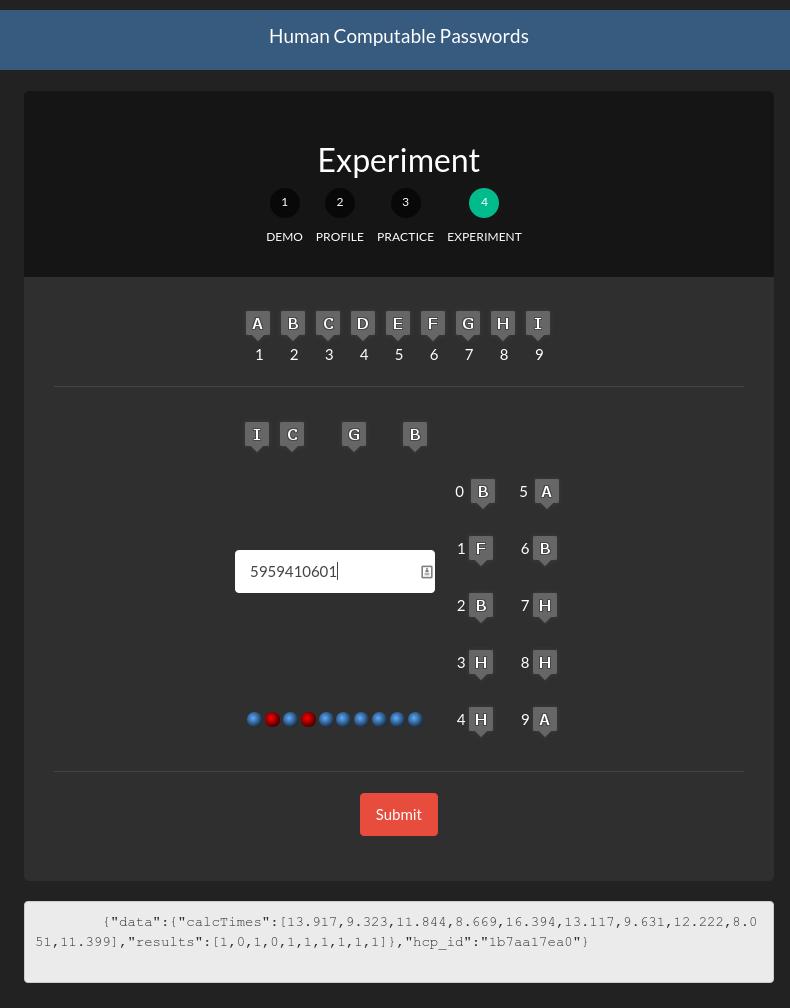
\includegraphics[width=\textwidth]{complete-experiment}
    \caption{The experiment screen seen after completing an experiment sample, ready to be submitted.}
    \label{complete-experiment}
\end{figure}

\par As for the storage of results a noSQL database called MongoDB is used. After completing a trial of the experiment a javascript object is stored in the database, \autoref{db-obj} shows an example of this object. Note the \emph{hcp\_id} field which is fetched from a cookie in the participants' browsers, making it persist across several trials. 

\par The views of the web application can be seen in \autoref{experiment-views} or by visiting the hosted experiment site at \url{hcp.sp1nakr.com}.

\begin{table}
\begin{tabular}{|c|c|}
    \hline
    hcp\_id & 1b7aa17ea0  \\ \hline
    occupation & Technology student \\ \hline
    age & 27 \\ \hline
    results & $[1,1,1,1,1,1,1,1,1,1]$ \\ \hline
    calcTimes & $[12.047,7.115,8.022,9.283,10.544,8.807,9.925,9.78,7.11,8.187]$ \\ \hline
\end{tabular}
\caption{Experiment object after completing a trial, as stored in the database.}
\label{db-obj}
\end{table}

\section{Results}

This section will present the results of the conducted experiment and investigate the characteristics of the data recorded. The focus will be on the calculation times and failure rate, which both are important factors in the resulting usability of the scheme, as discussed in \autoref{sec:usability}.
\par The observations made are not necessarily representative for all users, because of the relatively small number of samples ($342$ singlet digit challenges), but it is still interesting to investigate the consequences of the results. Even if the results show that the scheme achieves a lower level of usability than what are considered acceptable, it might still function well for some users with the right amount of practice. The limitations of the experiment will be discussed, in addition to results and the consequences of these.

\subsection{Calculation times.}
How fast a user is able to calculate the response to a single digit challenge is a concrete measure of the usability of the scheme. Figure \ref{histo-calctimes} shows the distribution of calculation times of all the experiment samples, the calculated average off all the $342$ trials are $10.922$ seconds. The median value is $10.104$ with standard deviation of $3.64$ which also can be observed in the figure. 
\par Recall \autoref{conjecture1} from \autoref{human-func}. The function $f$ (see definition \ref{fo-function}) used in this project is $(P,9,3)$-computable. The conjecture then defines the variable $\gamma_H$ for user $H$ as {\Large $\gamma_H = \frac{\hat t}{9}$}. 
\par The average $\gamma$ of all the participants are $\tilde \gamma = \frac{10.922}{9} = 1.214$. This is slightly higher than the $7.5$ seconds ($\gamma_H \le 1 $) Blocki~\cite{hcp-blocki} predict that users with moderate mathematical backgrounds should achieve. It is still not unreasonably high, and should not be a direct hindrance. Calculating a 10 character password would in example take $11 \cdot 10 = 110$ seconds, just short of 2 minutes, to calculate, 15 character would close in on 3 minutes. On average spending 2-3 minutes on calculating a password might seem like a lot, but a user concerned about the security of his accounts, might be willing to make this trade-off. Especially is the user is worried about putting his passwords in the hands of a online service to store persistently (e.g. \emph{lastpass.com}), might be willing to put quite some time into calculating his own passwords instead.
\par It is also relevant to study the evolution of each user in terms calculation times. Figure \ref{scatter-regression} illustrates the average calculation time for each $i$th trail per user. $i=1$ represent the average of the first calculation done by each user, $i=2$ the second calculation etc. The figure clearly illustrates that the averages decrease with practice. This could have been expected, since the users will be more and more familiar with the calculation procedure for each trial. The consequence of this observation is that the average calculation time, and consequently $\gamma$, would be significantly lower if the participants got more practice with the scheme before their results was recorded. Each participant averaged $30$ samples each, so it is not feasible to e.g. calculate the average after removing the 20 first calculations from each participant, as this would leave very few trials. The important goal of the experiment is though not to find a accurate average calculation time, but to verify that $\gamma_H \le 1$ is a reasonable for most users. It seems that the average most likely is somewhere between 9 and 11, depending on how long the users has been using the scheme, which is not severely limiting.

\begin{figure}
    \centering
    \begin{tikzpicture}
        \begin{axis}[width=\textwidth, xlabel=Calculation times in seconds. ,ybar, ymin=0, yticklabels={,,}]
            \addplot +[
                    hist = {
                        bins=20,
                        data min=3,
                        data max=20
                    },
                    fill=blue!60
                ]table [y index=0]{calcTimes.csv};

        \end{axis}
    \end{tikzpicture}
    \caption{Histogram showing the distribution of calculation times of all the recorded experiments. Sample size $342$ single digit challenges.}
    \label{histo-calctimes}
\end{figure}


\begin{figure}
    \centering
\begin{tikzpicture}
    \begin{axis}[
                enlargelimits=false,
                xlabel=Trial number: $i$,
                ylabel = Average calculation time in seconds.,
                width=\textwidth,
                ymin=4,
                ymax=18
        ]
        \addplot+[
                only marks,
                scatter,
                mark size=1.5pt
            ]
            table[meta=avg]
            {sum-avgs.dat};
        \addplot[
            domain=0:80,
            samples=3,
            very thick
        ]{12.56074424-0.06942622*x};
    \end{axis}

\end{tikzpicture}
\caption{Average calculation time of all participants' $i'th$ calculation sample, and the regression line of the averages. Sample size $342$, average samples per participant $31$.}
\label{scatter-regression}
\end{figure}


\subsection{Failure rate.}
Failure rate is a key characteristic of the scheme, as mentioned it is essential that a user is able to calculate passwords correctly for the scheme to function. How high the failure rate can be depends on how long passwords are used and how often a user can enter the wrong password without locking the account. A typical password protected site will allow a minimum of three strikes before the account is locked~\cite{10-strikes}. It is thus important that the probability of being "locked out" is small enough for it not to happen often, how often is of course subject to discussion.

\begin{observation}\label{obs:failrate}
    Average failure rate for all samples recorded in the experiment was measured to be $\tilde \lambda = 0.0584795321637$, approximately every one out of 17 single digit challenge was calculated wrong.
\end{observation}
This observation might not seem very unusual, but since a password consist of a sequence of calculation, it is required that the user calculate a given number of challenges consecutively without failure. It is thus more interesting to evaluate the probability of having at least one mistake in a complete password calculation sequence. It is also not unusual to enforce a password policy using a three-strike policy which will lock the account if three consecutive mistakes are made. Next, these probabilities are presented and discussed. 


The probability of having at least one mistake in a length $l$ password given the failure rate $\lambda$ is given by
\begin{equation}\label{eq:failrate}
    P(fail) = 1 - (1 - \lambda)^l
\end{equation}

Next, the probability of getting the account locked given a three-strike policy with the same password and failure rate is 
\begin{equation}\label{eq:lockrate}
    P(lock) = ( 1 - (1 - \lambda)^l )^3
\end{equation}


\begin{table}[h]
    \centering
\begin{tabular}{|c|c|c|c|c|}
    \hline
    Password length $l$ & $3$ & $5$ & $10$ & $15$ \\ \hline \hline
    $P(fail)$ & $0.1654$ & $0.2601$ & $0.4526$ & $0.5959$ \\ \hline
    $P(lock)$ & $0.0045$ & $0.0176$ & $0.0927$ & $0.2107$ \\ \hline
\end{tabular}
\caption{Probability of having at least one mistake in a length $l$ password given failure rate $\lambda = 0.0584795321637$ for each single digit challenge.}
\label{tbl:failrate}
\end{table}
 
\par Observation \ref{tbl:failrate} shows the probabilities of calculating a password wrong once and three times in a row. If a user wants to use a password of 15 characters, which is reasonable to assume since the scheme only produce digits, he will compute a faulty password nearly 60\% of the time. This limits the usability severely, since a user will more often than not, be unable to log in.
\par The probability of actually locking the account by miscalculating three passwords in a row, is lower but not significantly. With the same failure rate and password length, a user would break the three-strike rule approximately one out of five login attempts.

\par To illustrate this consequence in a extreme case, consider the \emph{very active} user from table \ref{users} in \autoref{sec:usability-model} which visits 10 different accounts every day. Such an user would eventually lock two accounts every day with password lengths of 15 characters, which of course is not acceptable.


\subsection{Improvement Measures.}
\par Blocki et al.~\cite{hcp-blocki} suggests a tweak to the scheme with the purpose of decreasing the calculation time while still ensuring resistance against dictionary attacks. The suggestion is to memorize another mapping $w:\mathbb{Z}_{10} \rightarrow \{x\}$ with $x$ being one of the $10000$ most common English words. Then after computing $f(\sigma(C))$ the user would apply $w$ giving the corresponding word to the digit. The point of doing this is to save time when calculating, but it also solves the problem with high failure rates. Blocki argues, it would be sufficient with 3-5 challenges. With this assumption that 3-5 calculations are enough, the scheme would function significantly better. 
\par Using the same example with the very active user, an account would be locked every 222nd login attempt with length 3 and every 57th with length 5. This would be be a huge improvement, actually making the scheme usable.

\par As discussed in \autoref{improving-usab} (and as implemented in \autoref{app}), the password length needed for different accounts may vary. By using shorter password for noncritical accounts, and only generate long password for the most critical, the average password length will be much lower than in the examples above. The scheme could then be tweaked by the user to fit specific needs, instead of requiring 10 or 15 characters in all password generated. 

\begin{remark}
    The author remarks that the findings related to failure rates might be too harsh since the participants was asked to calculate the challenges "as fast as possible", which might be the wrong approach. In a real world scenario it would be more important to calculate correctly. Though, the results clearly show that the failure rate is a relevant attribute worth investigating closer, as it might limit the usefulness of the scheme in real usecases.
\end{remark}



